% ************************************************
\chapter{Strucutral Aspects}\label{ch:Graph Theory} % $\mathbb{ZNR}$
% ************************************************
In this chapter we review basic graph theory and explain how these
terms are applicable in the context of biological neural networks. We
begin with the definition of directed graphs:

\section{Definitions \& Basics}

References for this chapter:
\url{http://nlab.mathforge.org/nlab/show/graph},
\url{http://nlab.mathforge.org/nlab/show/quiver}, \parencite{Bang-Jensen_Digraphs} 


%  \begin{defn}[Graph, Order] A \textbf{graph} is a pair of sets $G
% =(V,E)$, consisting of the \textbf{vertex set} $V(G)=V$ and the
% \textbf{edge set} $E(G)=E$, such that $E \subseteq V \times V$.  The
% number of vertices of a graph $G$ is its \textbf{order} $|G|$, the
% number of edges is denoted by $||G||$.  A graph of order $0$ or $1$ is
% called \textit{trivial}.
%   \end{defn}

%   The object of interest in my thesis will be directed pseudographs,
% but I will still have to think about how to
%   \begin{itemize}
%   \item call them, graphs, directed graphs, etc..
%   \item think about the weights(!!)
%   \item think about definitions
%   \end{itemize}

%   \bigskip




\begin{defn}[Directed graphs]
  A \textbf{directed pseudograph} $G$ consists of two finite \red{(,
    non-empty?)} sets $V$, the \textit{set of vertices} of $G$, and
  $E$, the \textit{set of edges} of $G$, and two maps
  \[
  s,t: E \to V,
  \]
  the \textit{source} and \textit{target functions} of $G$. A
  \textbf{directed multigraph} is a directed pseudograph without
  \textit{loops}, that is the map $d = (s,t):E \to V^2$ already maps
  maps to $V^2\setminus\Delta_V$, where $V^2 = V \times V$ denotes the
  cartesian product and $\Delta_V = \{(x,x)|x \in V\} \subseteq V^2$
  the diagonal. Similarily, a \textbf{directed loop graph} is a
  directed pseudograph where $d$ is injective. Finally, a
  \textbf{simple directed graph} can be defined as a directed
  pseudograph where $d$ is both injective and already maps to
  $V^2\setminus\Delta_V$.
\end{defn}

Thus, in simple directed graphs, neither parallel edges nor loops -
edges between the same vertex - are allowed, whereas directed
multigraphs and directed loop graphs admit one of them respectively.

\red{Say something about what "directed graph" means here.}

Given a directed graph $G$, we denote with $V(G)$ the set of vertices
of $G$ and call it the \textbf{vertex set} of $G$. Analogously, the
\textbf{edge set} $E(G)$ of $G$ denotes the set of edges of $G$. This
means, for a directed graph specified as $G = (V_G,E_G,s_G,t_G)$, we
have \[V(G) = V_G \quad \mathrm{and} \quad E(G) = E_G.\]


\begin{figure}
  % \includestandalone[width=\textwidth]{gfx/tikz/directed_graph_types}
  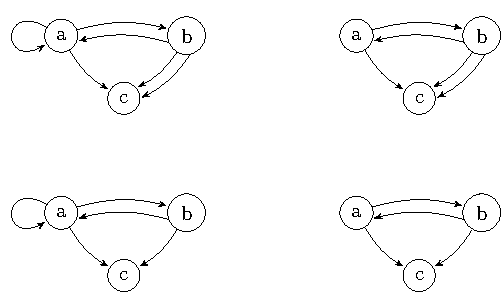
\includegraphics{gfx/tikz/directed_graph_types.pdf}
  \caption{From top left to bottom right, typical examples of the
    defined graph types: A) directed pseudograph, B) directed
    multigraph, C) directed loop graph D) simple directed
    graph.} \label{fig:M1}
\end{figure}


A \textbf{morphism} $\phi: G \to H$, between two directed graphs
$G=(V_G,E_G,s_G,t_G)$ and $H=(V_H,E_H,s_H,t_H)$, consists of a pair of
maps $\phi_V: V_G \to V_H$ and $\phi_E: E_G \to E_H$, such that
\[
s_H \circ \phi_E = \phi_V \circ s_G \mathrm{\quad and \quad} t_H \circ
\phi_E = \phi_V \circ t_G,
\]

that is such that the following diagram commutes:

\begin{align*} 
  \xymatrix@+=1.3cm{E_G \ar^{t_G}@<0.66ex>[d] \ar_{s_G}@<-0.66ex>[d]
    \ar^{\phi_E}[r] & E_H \ar^{t_H}@<0.66ex>[d]
    \ar_{s_H}@<-0.66ex>[d]\\ V_G \ar^{\phi_V}[r] & V_H}
\end{align*}

\bigskip

A morphism $\varphi: G \to H$, between two directed pseudographs $G$
and $H$ is an \textbf{isomorphism}, if the maps $\varphi_V: V_G \to
V_H$ and $\varphi_E: E_G \to E_H$ are bijective. Two directed
pseudographs are called \textit{isomorphic} if there exists an
isomorphism inbetween them.

\begin{remark}
  The last definition implies that, if there exists an isomorphism
  $\varphi: G \to H$, an isomorphism $\psi: H \to G$ can be
  found. This isomorphism is, of course, easily constructed via
  $\psi_V: V_H \to V_G, v \mapsto \varphi_V^{-1}(v)$, $\psi_E: E_H \to
  E_G, e \mapsto \varphi_E^{-1}(e)$.
\end{remark}

\begin{defn}[Weighted directed graphs]
  A \textbf{weighted directed graph} is a directed graph $G$ along
  with a mapping $\omega: E(G) \to \mathbb{R}$, called the
  \textit{weight function}. Similarily, a \textbf{vertex-weighted
    directed graph} is a directed graph with a mapping $\nu: V(G) \to
  \mathbb{R}$.
\end{defn}

\begin{remark} \red{(heavy draft)}, title: A directed graph category
for biological neural networks, in a bordered box?\\ Certainly, a
weighted directed pseudograph is the most fitting mathematical
modelling to the biological situation, since self connections and
multiple synapse are not only plausibel (source?) but the
rule. However there is one abstraction we can make by adding together
the synaptic weights - NEST is doing it..\\ Also think about
\textbf{inhibitory, excitatory}. Suggestion: edge weights $\omega:
E(G) \to \mathbb{R}^{+}$ \textbf{and} vertex weights $\nu: V(G) \to
\{-1, 1\}$. Synaptic weight $\mathrm{syn}(e)$ for edge $e$ is
then \[\mathrm{syn}(e) = \nu(s(e))\,\omega(e).\] Benefit: Synapse from
one neuron are either excitatory or inhibitory but not mixed as in
bio.
\end{remark}


\begin{remark}[Equivalent definiton for directed loop graphs]
  A directed loop graph $G$ can be equivalently defined as a pair of
  finite\red{(, non-empty?)} sets $V$, the \textit{set of vertices} of
  $G$, and $E \subseteq V^2$ the \textit{set of edges} of $G$. For an
  edge $(x,y) \in E$, we call $x$ the \textit{source} and $y$ the
  target of the edge $(x,y)$.

  Source and target functions are then uniquely determined as the
  projections on the first and second component, $s = \mathrm{pr}_1, t
  = \mathrm{pr}_2: E(G) \to V.$ Conversely, the edge set $E(G)
  \subseteq V^2$ can be determined from the source and target
  functions as $E:=\{(s(e),t(e)) | e \in E\}$. The trivial identities
  $(x,y) = (\mathrm{pr}_1(x,y),\mathrm{pr}_2(x,y))$ and
  $\mathrm{pr_1}(s(e), t(e)) = s(e)$ with $\mathrm{pr_2}(s(e), t(e)) =
  t(e)$ quickly verify the equivalence of the definitions.

  Given a directed loop graph $G$, we often assume the graph to be
  given in this form and write edges as $e=(x,y)$. Note that this
  concept is more complicated to introduce for directed pseudographs,
  since parallel edges $e$ and $e'$ should to be differentiated in the
  egde set of $G$, establishing the need for $E(G)$ to be a multi- or
  indexed set, notions we are trying to avoid in this document.
\end{remark}




% A given directed loop graph $G = (V,E,s,t)$, can always be
% represented by a canonical isomorphic directed loop graph $G' =
% (V,E')$, where $E':=\{(s(e),t(e)) | e \in E\} \subseteq V^2$. For a
% directed loop graph $G'$ in canonical form, the source and target
% functions $s',t'$ do not need to be specified, since they are uniquely
% determined as the projections on the first and second component, $s' =
% \mathrm{pr}_1, t' = \mathrm{pr}_2$. Wait, not so easy because
% multi-sets, however add synaptic strength of parallel edges to make
% directed loop-graphs! (Bang-Jensen)



From now on any \textit{directed graph} is assumed to be a directed
loop graph. Although most, if not all, concepts work for directed
pseudographs just as well, we want to start to heavily use the
canonical edge representation, which when talking about pseudograps
makes problems as mentioned before.

\begin{remark}[More Notation] 
  \red{- Check, do I really need this?} For a pair of vertex sets $X,Y
  \subseteq V(G)$ of a directed graph $G$ we write
  \[
  (X,Y)_G = \{(x,y) \in E(G) | x \in X, y \in Y \}
  \]
  for the set of edges with source in $X$ and target in $Y$. For
  vertex sets with a single element $X = {x}$, we also write $(x,Y)_G$
  and mean the edges with source $x$ and target in $Y$.
\end{remark}


\begin{remark}[In- and out-degree] 
  For a directed graph $G$ the \textbf{in-degree} $d^-_G(x)$ of a
  vertex $x$ is defined as the number of edges of $G$ with target $x$,
  that is
  \[
  d^-_G(x) = \left|(V(G),x)_G\right|.
  \]
  Similarily, the \textbf{out-degree} $d^+_G(x)$ of $x$ is defined as
  \[
  d^+_G(x) = \left|(x, V(G))_G\right|,
  \]
  the number of edges in $G$ with source $x$.
\end{remark}

\begin{remark}[Side]
  In some literature about directed graphs (Bang-Jensen), loops are
  \textit{not} counting towards the in- or out-degree of vertex. In
  the light of neural network however, we specifically want to count
  loops as well.
\end{remark}

A basic property of the in- and out-degree in directed graphs is that
number of in-degrees of every vertex, as well the sum of every
out-degree, equal the total number of edges:

\begin{proposition}
  In every directed graph $G$, we have
  \[
  \sum_{x \in V(G)} d^-(x) = \sum_{x \in V(G)} d^+(x) = | E(G) |.
  \]
\end{proposition}

\begin{proof}
  Since $(V(G),x)_G \cap (V(G),y)_G = \emptyset$ for $x \ne y$, we can
  write
  \[
  \sum_{x \in V(G)} d^-(x) = \left| \bigcup_{x \in V(G)} (V(G),x)_G
  \right| = \left| (V(G),V(G))_G \right| = | E(G) |.
  \]
  Analogously for the out-degree.
\end{proof}


\subsection*{Walks and distances}

Let $G$ be a directed graph \red{(what does it mean here?)}. A
\textbf{walk} $W$ in $G$ is an alternating sequence
$(x_1,e_1,x_2,e_2,x_3,\ldots,x_{n-1},e_{n-1},x_n)$ of of vertices
$x_i$ and edges $e_i$ from $G$, such that
\[
s(e_i) = x_i \quad \mathrm{and} \quad t(e_i) = x_{i+1}, \:\,
\mathrm{for}\, i=1,..,n-1,
\]
that is, such that the vertices are connected by the edges inbetween
them. We denote the set of vertices $(x_1,\ldots,x_n)$ of $W$ as
$V(W)$ and the sequence of edges $(e_1,\dots,e_{n-1})$ as $E(W)$
\red{(need it?)}.

The vertices $x_1$ and $x_n$ are called the \textit{end vertices} of
$W$ and we also say that $W$ is an $(x,y)$-walk. The \textbf{length}
of $W$ is defined as the length of the sequence of edges; a walk
consisting of only one vertex has length zero. \red{ colon, really?}


\begin{defn}[Distance]
  The \textbf{distance} of two vertices $x$,$y$ in a directed graph
  $G$ \red{(means?)}, is defined as the minimum length of an
  $(x,y)$-walk, if any such walk exists, otherwise
  $\operatorname{dist}(x,y)=\infty$. In short,
  \[
  \operatorname{dist}(x,y) = \inf \{|E(W)| \mid
  W\,\mathrm{is}\,(x,y)\mathrm{-walk}\}.
  \]
  \red{$|E(W)|$ is not explained. Necessary?}
\end{defn}

\begin{proposition}
  The distance function $\operatorname{dist}: V(G) \times V(G) \to
  \mathbb{N}$ of a directed graph $G$ satisfies the triangle equality,
  \[
  \operatorname{dist}(x,z) \le \operatorname{dist}(x,y) +
  \operatorname{dist}(y,z), \:\: \mathrm{for}\:\, x,y,z \in V(G).
  \]
\end{proposition}

\begin{proof}
  Let $x,y,z$ be vertices in $G$. If either no $(x,y)$-walk or
  $(y,z)$-walk exists, the inequality holds by definition. Other wise,
  let $W$ be an $(x,y)$-walk of minimal length and let $U$ be a
  $(y,z)$-walk of minimal length. Certainly, by concatenating $W$ and
  $U$ we obtain an $(x,z)$-walk of length $|E(W)| + |E(U)| =
  \operatorname{dist}(x,y) + \operatorname{dist}(y,z)$, proofing
  that \[ \operatorname{dist}(x,z) \le \operatorname{dist}(x,y) +
  \operatorname{dist}(y,z).
  \]
\end{proof}





%   \begin{defn}[Neighbour, adjacent] Two \textbf{vertices} $x,y \in
% V(G)$ of $G$ are called \textit{adjacent} or \textit{neighbours} if
% there is an edge between $x$ and $y$, $(x,y) \in E(G)$. Two
% \textbf{edges} $e \neq f$ are \textit{adjacent} if they have an end in
% common.
%   \end{defn}


More to do:

\begin{itemize}
\item summarize category of directed (weighted) pseudographs
\item weights!
\item vertices will also be called nodes and neurons, edges will also
  be connections or synapses.
\item subgraphs
\item vertex set, edge set $E(G), V(G)$.
\item $\omega(e)$ is weight, connection strength or synaptic weight
  (as a side remark
\item extend to category of weighted directed pseudographs
  (isomorphisms)
\item path
\item adjacency matrix
\item converses of graph related to opposite category?
\item in- and out-degree
\item triangle inequality for distance, $\mathrm{dist}(x,z) \leq
  \mathrm{dist}(x,y) + \mathrm{dist}(y,z)$
\end{itemize}

\bigskip

\section{Random Graph Theory}

For this chapter, as it is common and practical when talking about
random graphs, we move away from the the abstract notion of graphs and
their equivalence classes and consider \textit{labeled graphs}, where
the edge set of a graph with $n$ vertices takes the form $V =
\{1,\ldots,n\}$.




\subsection{Erd\H{o}s-R\'{e}nyi graphs}

References: Newman, Erdos1960, Erdos1959, Gilbert1959, 
Wikipedia, \parencite{West_Graph-theory}
		
		
\begin{defn}[Terms used]
  Graphs with $n$ vertices: $G^n = \{G| G\,\mathrm{is\,
    graph\,(means??)},\, |V(G)| = n\}$
\end{defn}
		
\begin{remark}[Expected number of edges in a directed Erd\H{o}s-R\'{e}nyi graph (DERG)]
  $X: G^n \to \mathbb{R}, G \to |E(G)|$, discrete random variable,
  with probability distribution $G(n,p) =\operatorname{B}(n^2,p)$,
  binomial distribution. That is, distribution of $X$ via probability
  mass function $P(X=k) = {{n^2} \choose k} p^k\,(1-p)^{n^2-k}$. Thus
  $\operatorname{E}(X)$ equals expect edges in DERG. We have of
  course, since $G(n,p)$ binomial,
  \[
  \operatorname{E}(X) = pn^2. \mathrm{\:(if\,self-edges!)}
  \]
  Then, of course, the \textbf{mean in-}  and \textbf{out-degree} is \[ \langle
  d^{\mathrm{in}} \rangle = \langle d^{\mathrm{out}} \rangle =
  \frac{\langle |E(G)| \rangle}{|V(G)|} = np.\] \textit{Does this make
    sense? Define everything properly!!}
\end{remark}



% From Graph clustering - Satu Elisa Schaeffer - 2007
% 
% [84] P. Erdos, A. Rényi, On random graphs I, in: Selected Papers
% of Alfréd Rényi, vol. 2, Akadémiai Kiadó, Budapest, Hungary,
% 1976, pp. 308–315. First publication in Publ. Math. Debrecen
% 1959.
% [85] P. Erdos, A. Rényi, On the evolution of random graphs,
% in: Selected Papers of Alfréd Rényi, vol. 2, Akadémiai Kiadó,
% Budapest, Hungary, 1976, pp. 482–525. First publication in
% MTA Mat. Kut. Int. Közl. 1960.





%%% Local Variables: 
%%% mode: latex
%%% TeX-master: "../ClassicThesis"
%%% End: 
